\section{Question 1: Measurement}
\textit{Discuss levels on which variables could be measured. How the level of measurement influences the choice of statistical tools? (Hint: While answering this question, consult Chapter 8 of the book).}

\section{Question 2: Experimental Design}
\textit{In an experimental design, what do aims Reliability, Validity and Importance mean? Which actions should be taken to maximize measurements' reliability and validity?}
\hspace{0pt} \\
\\
Reliability and validity are two fundamental aspects of any experimental design. The idea and purpose behind these are to control the systematic measurement errors, and thereby reducing the inconsistency of the measurement \citep[p. 44-48]{Design}. The aim of importance is simply whether a study or research is of importance. That is, however, a rather subjective matter. Time also changes what is found as of importance. If research is neither valid nor reliable, it cannot possibly be of importance \citep[p. 54]{Design}.

Reliability refers to the consistency of a measure. For a measure to be reliable, it must be replicable and produce the same results under same conditions. There are several ways to estimate reliability of a measurement instrument. \textit{Test-retest} reliability is the ability to repeat the measurements across different points in time. This type of reliability wants to achieve the same results each time \citep[p. 47]{Design}. Another method to measure the consistency (reliability) is the \textit{split-half} method. E.g. in a questionnaire consisting of 10 items, the method splits it into two groups of 5 items. For each half, a score is calclulated, and then the two halves are compared. If they are reliable, the two halves should have a large correlation. \textit{Cronbach’s alpha} is the average of split correlations, and an alpha value of 0.8 or above is accepted to be reliable \citep[p. 48]{Design}.

Validity is essentially whether the measurements actually measure what it is supposed to, or what it claims to measure. There are many types of validity. One of them is \textit{content validity}. The content of a test should cover the content of the construct it was designed for. It is obtained by carefully selecting the “right” items to be included in a test \citep[p. 44-46]{Design}. Another type of validity is \textit{criterion validity}, which in essence is whether a measurement accurately predicts an outcome measure, e.g. by correlating scores with other known measures of the construct \citep[p. 46-47]{Design}. A third type of validity is \textit{factorial validity}. It is based on factorial analysis, which is a statistical technique to find out which items, or questions in a questionnaire, that are related. It is used when designing proper questions for a questionnaire, where sub-components should make intuitive sense and this is where factorial validity can be used \citep[p. 47]{Design}. Other types of validity exist, but are not included in this mini-project. However, the two most common forms of validity is \textit{internal} and \textit{external validity}. The internal validity concerns following the principles of cause and effect, which is evidence that the manipulation of the independent variable had an effect on the outcome result. As said, the purpose of validity is to minimize and control the potential errors, and there are many factors that can threat the internal validity. Eight of the most common threats to internal validity are as follows \citep[p. 58-62]{Design}:

\begin{itemize}
\item \textbf{Group threats}: differences in groups at the start of the study .
\item \textbf{Regression to the mean}: participants produce very high/very low scores by chance.
\item \textbf{Time threats}: participants' behavior may change over time.
\item \textbf{History}: unrelated to the manipulation of the independent variable, events can occur simultaneously with the experiment, and it becomes and alternative explanation to the change in participants’ behavior. 
\item \textbf{Maturation}: participants’ behavior may change due to natural development (i.e. children). 
\item \textbf{Instrument change}: changes due to change of instrument, e.g. an interviewer gets more tired or bored during the day, or maybe becomes more excited. 
\item \textbf{Differential mortality}: participants may drop-out, making it hard to compare pre- and post-tests, and leaving behind participants’ with systematic differences.
\item \textbf{Reactivity and Experimenter Effects}: measuring participants’ behavior may affect their behavior. The experimenter can bias the results in the way they interact with the participants. Can be minimized using the “double-blind” technique, in which the experimenter and participants are unaware of the experimental hypothesis.
\end{itemize} 

The external validity is more a question of how the measurements can be generalized. Here can be mentioned two types of threats to the external validity, which reduces the generalization \citep[p. 62]{Design}. The first threat is \textit{over-use of special participant groups}, e.g. when the participants are voulenteers, they might be more engaded in the study than non-voulenteers, and so they do not have same characteristics as the general population \citep{Lard}. The second is \textit{restricted number of participants}, where experiments often use too few participants to attain statistical significance, which is in particular also a thread to the reliability \citep[p. 62]{Design}.

To maximize the reliability, experimenters should describe specific definitions on what is being measured \citep[p. 57]{Design}. Isolating causal factors, and minimize alternative explanations will increase the validity \citep[p. 62]{Design}. Running pilot tests before the real data-collection, as well as having experts reviewing the content, can reveal some errors and problems which can be adjusted to increase the reliability and validity of a study \citep[p. 407-408]{ResearchMethods} \citep{NCTI}. Many potential unsystematic variations can be eliminated by randomization, in which participants are randomly allocated in the parts of the study \citep[p. 24]{Design}.

\section{Question 3: Analysis of Presented Data}
\textit{Analyze and present data gathered by a group of MED10 students for their semester project. Use available materials as a guideline and inspiration. Follow the document DAEV-ANOVA-exercises.pdf, and be sure to make all statistical tests mentioned there and to answer each of the points. Do all needed calculations and make all illustrative figures in Matlab.}

\subsection{Repetition: t-test}
% DESCRIPTION FOR POINT 1.1 -----------------------------------
\noindent\colorbox{light-gray}{\begin{minipage}{0.98\textwidth}
\textbf{1.1.} In a test of how gaming performance was affected by different kinds of feedback, 10 participants were measured. All participants played the game twice, once with auditory, and once with visual feedback. The type of feedback given first was counter-balanced across the group. The table below displays the measured time (in seconds) it took for the gamers to complete the final level of the game for the two conditions.
\end{minipage}}

% QUESTION 1.1 (1) --------------------------------------------
\noindent\colorbox{lighter-gray}{\begin{minipage}{0.98\textwidth}
\begin{enumerate}[label=\textbf{(\arabic*)}]\setcounter{enumi}{0}
	\item Should a one or two-tailed test be used if we want to know if there is a significant difference in gaming time between the two types of feedback? How many degrees of freedom?
\end{enumerate}\end{minipage}}

% ANSWER ------------------------------------------------------
\hspace{0pt} \\
In this test we are looking for a difference in the gaming time between the two types of feedback (auditory and visual). This means we do not have a specific hypothesis, e.g. that visual feedback would give a shorter gaming time. The tests should instead tell us if one or the other type of feedback is best. The null-hypothesis then states that there is no difference between auditory and visual feedback. We have now conducted that the test we are looking at is non-specific, thus we need to use a two-tailed test, where each tail would tell us if one or the other type of feedback would give us a shorter gaming time \citep[pp. 155-156]{Design}.

For each of the two samples of the feedback types 10 persons were tested giving a total of 20. The degrees of freedom for the overall test is thus the sum of the sample sizes minus one for each sample. The degrees of freedom for the samples are then 18 or 9 for each sample.

% QUESTION 1.1 (2) --------------------------------------------
\hspace{0pt} \\
\noindent\colorbox{lighter-gray}{\begin{minipage}{0.98\textwidth}
\begin{enumerate}[label=\textbf{(\arabic*)}]\setcounter{enumi}{1}
	\item Use the correct t-test and answer the question whether there is a significant difference (=.05).
\end{enumerate}\end{minipage}}

% ANSWER ------------------------------------------------------
\hspace{0pt} \\
Before we can do a t-test to test for a significant difference, we have to make sure that the samples come from normal distributions with a homogeneity of variance. First we test for homogeneity of variance between the two samples (auditory and visual feedback) using Bartlett's test. Here we assume that the population from which the two samples came are normal distributed. In the figure \ref{fig:2-1-1_vartestn} we see the statistics with a p-value supporting the null-hypothesis that the two samples do in fact have a homogeneity of variance. In the corresponding box plot, we can see that both samples have the approximately same properties such as the median and the inter-quartile range. These properties also suggests that the variances might be similar.

\begin{figure}[t]
	\centering
	\begin{subfigure}[t]{0.48\textwidth}
		\includegraphics[width=\textwidth]{fig/{2.1.1_vartestn_stats}.png}
		\caption{Statistics}
		\label{subfig:2-1-1_stats}
	\end{subfigure}
	\begin{subfigure}[t]{0.48\textwidth}
		\includegraphics[width=\textwidth]{fig/{2.1.1_vartestn_boxplot}.png}
		\caption{Boxplot}
		\label{subfig:2-1-1_boxplot}
	\end{subfigure}
	
	\caption{\textit{{\footnotesize Results from a Bartlett's test for equal variances. In \ref{subfig:2-1-1_stats} the p-value indicates that difference in the variances from the two samples are non-significant at the 0.05 level. The plot in \ref{subfig:2-1-1_boxplot} shows that the samples look very much alike with almost equal medians and inter-quartile ranges.}}}
	\label{fig:2-1-1_vartestn}
\end{figure}

Next we want to ensure that both samples come from a normal distributed population. For this we use the Kolmogorov-Smirnov test, where we standardize our samples and test for the null-hypothesis that the two samples come from standard normal distributions. The test yields the values $p=0.9811$ and $p=0.9897$ supporting the null-hypothesis.

Using a paired t-test on the two matched samples gives a p-value of $p=0.0319$ indicating that there is in fact a significant difference between the two types of feedback given (auditory and visual). With an alpha of $\alpha=0.05$ we can clearly determine that auditory feedback does not give the same gaming time as with visual feedback.

With all that said we have to take into account that we only have sample sizes of $N=10$. This means that even though the t-test rejects the null-hypothesis that there is no difference between the two types of feedback, it can be difficult to determine if it actually is the type of feedback that makes the difference and not some other factors. Andy Field \citep{Design} suggests that because a sample of a size beneath $N=30$ is messy, it can be difficult to determine.

% DESCRIPTION FOR POINT 1.2 -----------------------------------
\hspace{0pt} \\
\noindent\colorbox{light-gray}{\begin{minipage}{0.98\textwidth}
\textbf{1.2.} Download the zip archive 10ml883-data.zip containing text files with ratings on engagement from different experimental conditions as collected by group 10ml883. Start by importing the Engagement ratings for mouse and keyboard interfaces, as reported after 5 and 30 minutes of playing. Perform a t-test to compare if there is a difference in the rating of the intellectual engagement after 5 and 30 minutes of play.
\end{minipage}}

% QUESTION 1.2 (1) --------------------------------------------
\noindent\colorbox{lighter-gray}{\begin{minipage}{0.98\textwidth}
\begin{enumerate}[label=\textbf{(\arabic*)}]\setcounter{enumi}{0}
	\item What type of t-test should you use? Independent samples or paired?
\end{enumerate}\end{minipage}}

% ANSWER ------------------------------------------------------
\hspace{0pt} \\
If we assume that both samples are taken from observing the same 19 participants twice, the two samples are then dependent of each other. This means that we cannot use an independent t-test but instead we use a dependent paired t-test.

% QUESTION 1.2 (2) --------------------------------------------
\hspace{0pt} \\
\noindent\colorbox{lighter-gray}{\begin{minipage}{0.98\textwidth}
\begin{enumerate}[label=\textbf{(\arabic*)}]\setcounter{enumi}{1}
	\item What probability is there of obtaining these particular mean values purely by chance?
\end{enumerate}\end{minipage}}

% ANSWER ------------------------------------------------------
\hspace{0pt} \\
By following the same steps as above, we first need to validate that the samples have a homogeneity of variance and come from a normal distributed population. Testing for homogeneity of variance we get the results presented in figure \ref{fig:2-1-2_vartestn}. As we can see it seems that that the two samples do not have very similar variances giving us a problem when trying to use the t-test. If we then test for normal distribution of the two samples on 5 minutes and 30 minutes we get $p=0.0285$ and $p=0.0573$ correspondingly. These values indicates that the sample on 5 minutes does differ from a standard normal distribution while the 30 minutes sample does not. Again this would make a t-test less valid.

Doing the actual t-test will yield a p-value of $p=0.0031$ indicating a difference in intellectual engagement caused by the amount of time playing the game, i.e. 5 minutes or 30. However, since the validations of homogeneity of variance and of normal distribution, we might make a mistake stating that playing-time do make a difference.

\begin{figure}[h]
	\centering
	\begin{subfigure}[h]{0.48\textwidth}
		\includegraphics[width=\textwidth]{fig/{2.1.2_vartestn_stats}.png}
		\caption{Statistics}
		\label{subfig:2-1-2_stats}
	\end{subfigure}
	\begin{subfigure}[h]{0.48\textwidth}
		\includegraphics[width=\textwidth]{fig/{2.1.2_vartestn_boxplot}.png}
		\caption{Boxplot}
		\label{subfig:2-1-2_boxplot}
	\end{subfigure}
	
	\caption{\textit{{\footnotesize Results from a Bartlett's test for equal variances. The p-value seen in \ref{subfig:2-1-2_stats} tells there is a significant difference between the variances of the two samples. In boxes in \ref{subfig:2-1-2_boxplot} also shows a significant difference in the distribution of the observations in the two samples.}}}
	\label{fig:2-1-2_vartestn}
\end{figure}

% QUESTION 1.2 (3) --------------------------------------------
\hspace{0pt} \\
\noindent\colorbox{lighter-gray}{\begin{minipage}{0.98\textwidth}
\begin{enumerate}[label=\textbf{(\arabic*)}]\setcounter{enumi}{2}
	\item Is there a significant difference?
\end{enumerate}\end{minipage}}

% ANSWER ------------------------------------------------------
\hspace{0pt} \\
As explained above in 1.2 (2), yes there seems to be a significant difference.

% DESCRIPTION FOR POINT 1.3 -----------------------------------
\hspace{0pt} \\
\noindent\colorbox{light-gray}{\begin{minipage}{0.98\textwidth}
\textbf{1.3.} Now import the ratings for Wiimote after 30 minutes of playing. Proceed to explore the differences in Physical engagement between players using the mouse and keyboard interfaces, as compared to those using the Wii-mote. Test for differences in the ratings of Physical engagement between the two groups after 30 minutes of play.
\end{minipage}}

% QUESTION 1.3 (1) --------------------------------------------
\noindent\colorbox{lighter-gray}{\begin{minipage}{0.98\textwidth}
\begin{enumerate}[label=\textbf{(\arabic*)}]\setcounter{enumi}{0}
	\item What type of t-test should you use? Independent samples or paired?
\end{enumerate}\end{minipage}}

% ANSWER ------------------------------------------------------
\hspace{0pt} \\
Again we assume that the two samples uses the same 19 participants, thus the samples are dependent of each other. Therefore we must use a dependent/paired t-test.

% QUESTION 1.3 (2) --------------------------------------------
\hspace{0pt} \\
\noindent\colorbox{lighter-gray}{\begin{minipage}{0.98\textwidth}
\begin{enumerate}[label=\textbf{(\arabic*)}]\setcounter{enumi}{1}
	\item What probability is there of obtaining these particular mean values purely by chance?
\end{enumerate}\end{minipage}}

% ANSWER ------------------------------------------------------
\hspace{0pt} \\
Following the exact same steps we find that there is not any significant difference in the variances of the two samples given the data presented in figure \ref{fig:2-1-3_vartestn}. This is derived from the p-value of $p=0.788$ that clearly lies above the $0.05$ significance level. The test for normal distribution shows us that with the p-values of $p=0.1131$ and $p=0.1512$ the corresponding samples of the mouse \& keyboard and the Wii are deemed to belong to a normal distributed population.
Now we can perform the t-test between the two samples, which will give us a result of $p=0.00044$ clearly indicating a significant difference in physical engagement caused by changing the type of controller, i.e. mouse \& keyaboard or Wii.

\begin{figure}[h]
	\centering
	\begin{subfigure}[h]{0.48\textwidth}
		\includegraphics[width=\textwidth]{fig/{2.1.3_vartestn_stats}.png}
		\caption{Statistics}
		\label{subfig:2-1-3_stats}
	\end{subfigure}
	\begin{subfigure}[h]{0.48\textwidth}
		\includegraphics[width=\textwidth]{fig/{2.1.3_vartestn_boxplot}.png}
		\caption{Boxplot}
		\label{subfig:2-1-3_boxplot}
	\end{subfigure}
	
	\caption{\textit{{\footnotesize Results from a Bartlett's test for equal variances. Here the p-value in \ref{subfig:2-1-3_stats} indicates there is no significant difference in the variances, even though the boxes in \ref{subfig:2-1-3_boxplot} shows a very dissimilar distribution of the two samples.}}}
	\label{fig:2-1-3_vartestn}
\end{figure}

% QUESTION 1.3 (3) --------------------------------------------
\hspace{0pt} \\
\noindent\colorbox{lighter-gray}{\begin{minipage}{0.98\textwidth}
\begin{enumerate}[label=\textbf{(\arabic*)}]\setcounter{enumi}{2}
	\item Is there a significant difference?
\end{enumerate}\end{minipage}}

% ANSWER ------------------------------------------------------
\hspace{0pt} \\
As derived in 1.3 (2) there is a significant difference.
\subsection{Multiple Comparisons}
While t-test allows for the testing for cohesion between two mean values, it can often be insufficient when trying to calculate mean values of multiple test statistics. If more than two mean values are to be calculated, it must be done with pairwise testing. Every test increases the risk of committing type 1 errors i.e. accidentally rejecting a hypothesis that is actually true. Given a 5\% level of significance, the risk is thus 5\% per test. Therefore, if five mean values are to be tested (m1=m2=m3=m4=m5), the number of required tests would be 10, because all combinations must be executed. The combinatory conditions are calculated as follows:

\begin{equation}
\binom{n}{m} = {\frac{n!}{(m(m-n)!)}} 
\end{equation}\\
Meaning we will have the following amount of combinations:

\begin{equation}
\binom{5}{2} = {\frac{5!}{(2(5-2)!)}} = 10 
\end{equation}\\
This entails that every combination increases the probability of type 1 errors, and that the aggregated probability that type 1 error will be present in at least one of the tests is:

\begin{equation}
1-0,95^{10}= 1-0,599 = 40,1\%
\end{equation}\\
Hence, the probability  that at least one type 1 error will be present is approximately 40,1\%. The risk of committing a type 1 error will thus, increase explosively when the t-test is applied to mean-value comparisons of more than two populations.
\\

\subsection{Analysis of Variance (ANOVA)}
This increased risk can be very damaging for the credibility of any test; therefore it may be beneficial to eliminate as many confounding factors as possible. An \textit{analysis of variance}-test (ANOVA) may advantageously be used, as it is capable of comparing several mean values at once, and computing the variance.  To use ANOVA, one must apply the variance within each population as well as the variance between the populations. The formula for the 1-way ANOVA-test, also referred to as F-test, can thus be written:\\

\[F=\frac{between-group-variables}{within-group-variables}\]
\\
Thereby testing the mean value simultaneously rather than pairwise.
In the exercise (\textit{Design and Analysis of Experiments V: Exercies} by Sofia Dahl) three painkillers have to be compared to each other along with a placebo-version. Hence, there are four mean values that must be compared.  Instead of using the painkiller-data, we will analyse the data acquired by the 10th Semester group with a multiple comparison of means using the ANOVA-test, just like we have done in the previous assignments.
Since there are quite many dimensions of the aforementioned dataset, it is necessary to restrict ourselves to a few examples. Similar tests can be performed for all seven formats of engagement included in the data. But such a review would be comprehensive. If all combinations were to be tested we would have to test all of the three methods (MK, Wii and HMD) seven times, as well as seven times for each of the three time-entries (5,15 and 30) which would aggregate a total of 42 tests.
It is appropriate both logically and feasibly to start out with expanding the tests from exercice 1.2 and 1.3 to also include \textit{intellectual engagement for Mouse and Keyboard} after 15 minutes, and \textit{Physical engagement} for Head Mounted Display (HMD) after 30 minutes. Thus we have added an extra mean value that must be testet in the two tests, therefore we will use the one-way analysis of variance (ANOVA1 in MATLAB).\\

When using the ANOVA test a number of assumptions need to be fulfilled:
\begin{enumerate}
\item{The samples are normally distributed}
\item{The samples have the same variance (homogeneity of variance)}
\item{The samples are independent}
\end{enumerate}

Violations of assumption (1) can be acceptable, depending on how close the distribution is to the normal.
Violations of assumption( 2) will lead to inaccurate F-statistics. If the variances are significantly different, we can try to correct the problem by transforming the data or do a non-parametric test.
If assumption (3) is violated the F-statistics cannot be assumed to have an F-distribution. This means an increased probability of type II errors. 
Assumption (1) and (2) can be tested, whereas we have to look at the data in order to determine whether assumption (3) is a good assumption or not. In the case of the data from the 10th semester project, the samples cannot be assumed to be independent because it is the same 19 test subjects, that generates all the data. Hence, we need a new assumption:
(3a) Sphericity – the relationship between one pair of conditions is similar to the relationship of another pair of conditions \citep{Field_a}.
This assumption can be tested with the Mauchly’s test, which test the hypothesis, that the variance af the difference between conditions are equal \citep{Design}. Unfortunately we did not succeed in running this test in MATLAB, as the function is unknown. 
When using the repeated ANOVA, the test-statistics are generated using the variance within treatment and the variance between treatments.



\begin{figure}[h]
	\centering
	\begin{subfigure}[h]{0.48\textwidth}
		\includegraphics[width=\textwidth]{fig/{intellectualMK_testvalue}.png}
		\caption{Statistics}
		\label{IntellectMKtestVal}
	\end{subfigure}
	\begin{subfigure}[h]{0.48\textwidth}
		\includegraphics[width=\textwidth]{fig/{boxplotMK}.jpg}
		\caption{Boxplot}
		\label{intellectMK}
	\end{subfigure}
	
	\caption{{\footnotesize \textit{(a) Statistics shows the sum of squares (SS) which is the sum of the deviation in the power of 2, and degrees of freedom (DF) which is the number of “free” values that can be varied. The Mean Squares (MS) gives the average of the sum of squares SS/quantity, while the F-statistic (F) is the test statistic i.e. the measurements of the sample.The P-value (Prob$>$F) is The applied statistical probability that H0 is true in accordance with the f-statistic. (b) shows the notched boxplots generated by the test.}}}
	\label{ANOVA_1}
\end{figure}

In question 1.2 we tested the two samples (after 5 and 30 minutes) for normality, and we again perform the KS-test on the sample after 15 minutes. The KS-test shows, that we cannot reject the hypothesis, that the sample is normally distributed. As seen in the resulting figures of the ANOVA-test (fig. \ref{ANOVA_1}) we get a notched boxplot for the intellectual engagement after 5, 15 and 30 minutes. Although it is apparent that the medians are located similarly around 4 in the three groups, there are some considerable differences between them. After 5 minutes the grading ranges from 1 to 4, while after 15 and 30 minutes they range from 3 to 5. The notches in the figures specify the confidence interval (CI) around the mean, and it can tell us something about variance within each group. As previously specified one of the assumptions and requirements for the ANOVA-test is that there is similar variance (homogeneity of variance).  Although the variance after 5 and 15 minutes appears to be close to each other, the variance after 30 is less. The assumption of variance-cohesion can be tested with a Levene- variance test (vartestn in MATLAB), and the p-value from this test is 0,055 (5,5\%), hence we cannot reject that the three groups have the same variance.\\

The ANOVA table (fig. \ref{ANOVA_1}, (a) Statistics) generated by the one-way ANOVA-test generates an F-test statistic of 10,64 which gives a P-value of 0,0001 (0,001\%) which is way below our 5\% level of significance. Thus we can reject the null-hypothesis that there has been given similar grades for intellectual engagement after 5, 15 and 30 minutes.

\begin{figure}[h]
	\centering
	\begin{subfigure}[h]{0.48\textwidth}
		\includegraphics[width=\textwidth]{fig/{physical_testvalue}.png}
		\caption{Statistics}
		\label{PhysicalMKtestVal}
	\end{subfigure}
	\begin{subfigure}[h]{0.48\textwidth}
		\includegraphics[width=\textwidth]{fig/{BoxplotPhysical}.jpg}
		\caption{Boxplot}
		\label{PhysicaltMK}
	\end{subfigure}
	
	\caption{\textit{{\footnotesize (a) ANOVA Table and (b) Boxplot of the grades given for Physical Engagement after 30 minutes using the three types of controllers (mouse and keyboard, Wii and head mounted display).}}}
	\label{ANOVA_1.1}
\end{figure}

Figure \ref{ANOVA_1.1} shows the box plot for the grades given for Physical Engagement after 30 minutes using the three types of controllers. The median for HMD and MK are both 2, while Wii have a median of 3. The grades given range from 1 to 5 for both HMD and Wii, while MK only has one observation as high as 4 (in the boxplot it is regarded as an outlier). The notches indicate that the variance of the grades for HMD and Wii is larger than for MK. However, a variance test reveals a p-value of 0.905 indicating that we cannot reject the null-hypothesis of equal variance in the three samples. In question 1.3 we tested the two samples (physical engagement after 30 minutes for MK and Wii) and we test the last sample (HMD) as well and find that we cannot reject the hypothesis of normality. Hence, we continue with the ANOVA-test. This reveals an F-statistic of 7.31 which corresponds with a p-value of 0.0015 in the F-distribution with 2 DF. With a 5\% level of significance we reject the null-hypothesis that the three controllers are given the same score regarding physical engagement after 30 minutes.\\

A two-sided analysis of variance can test the effect of two factors simultaneously. The two-way ANOVA-test is performed for intellectual engagement after 5, 15 and 30 minuts for each of the three types of controllers. Hence, we test each factor (time and type of controller) alone (main effects) as well as the two factors combined (interaction). Thus we test if there is equal mean across time and type of controller as well as the interaction between them.

\begin{figure}[h]
	\begin{center}
		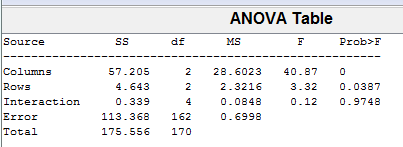
\includegraphics[height=3cm]{fig/anova2_testvalue.png}
		\caption{\textit{{\footnotesize Results for the two-sided ANOVA-test (anova2 in MATLAB) on intellectual engagement after 5, 15 and 30 minutes for each of the three types of controllers (mouse and keyboard, Wii and head mounted display).}}}
		\label{ANOVA_2}
	\end{center}
\end{figure}

The test (fig. \ref{ANOVA_2}) provides an F-statistic of 40.87 regarding the test across the columns (i.e. time). Hence, we can reject the hypothesis of equal mean grades for intellectual engagement after 5, 15 and 30 minutes. The test across the rows (types of controllers) provides an F-statistic of 3.32. In the F-distribution with 2 DF this corresponds with a p-value of 0.0387. With a 5\% level of significance we reject the hypothesis of equal mean for the three types of controllers. The last test has an F-statistic of 0.12 and a corresponding p-value of 0.9748. This provides evidence that there is no interaction between time and controller type in the grades given for intellectual engagement.